\documentclass[12pt]{article}
\usepackage[utf8]{inputenc}
\usepackage{amsmath}
\usepackage{amssymb}
\usepackage{graphicx}

\title{Math/CS 471 \\ Scientific Computing \\ HW5}
\author{Brian Kimbrell, Sandesh Timilsina}
\date{\today}

\begin{document}
\maketitle
\clearpage

\section{Mathematical Model}

Our system of ODE's is a model that describes a flock of birds. We have $N$ birds and we'll let
$$B_k(t) = (x_k(t),y_k(t)), k \in [1,N]$$

Where $B_k(t)$ is the $x$ and $y$ coordinates of the $k$th bird at time $t$.
Recall our general form of an ODE.
$$y(t)^\prime = f(t,y(t))$$

Here our right hand side function is the sum of all the forces on each bird, which depends on it's current location. We'll begin with just four different forces.
$$f(t,B(t)) = F^{food}(t,B(t)) + F^{follow}(t,B(t)) + F^{flock}(t,B(t)) + F^{repel}(t,B(t))$$
\begin{itemize}
    \item[$F^{food}$]  This will represent the tendency for the flock leader to chase a piece of food.
    Let $C$ define the location of the food at time $t$.
    $$C(t) = (x_c(t),y_c(t))$$
    We want to minimize the distance from the food to the lead bird, so we have
    $$F^{food}_1(t,(B(t)) = \gamma_1(C(t)-B_1(t))$$
    Where $\gamma_1$ is some positive constant that dictates who attracted the lead bird is to it.
    Note that this force effects only the lead bird, so in our implementation $F^{food}$ will be a $N \times 2$ matrix who's first row will be the only \textit{non zero} row.
    
    \item[$F^{follow}$] This will represent the tendency for the flock to follow the leader. We want to minimize the distance from the lead bird to each of the other birds so we define
    $$F^{follow}_k(t,B(t)) = \gamma_2(B_1(t) - B_k(t)), k \in [2,N]$$
    Where $\gamma_2$ is some positive constant the dictates how charismatic the lead bird is.
    Note here how this force effects all birds \textit{except} the lead bird. This means $F^{follow}$ will have \textit{zeros} in it's first row.
    
    \item[$F^{flock}$] This will represent the tendency for birds to flock as closely together as possible. Each bird will want to be as close to the center of the flock as possible. We'll define the center of the flock as 
    $$\Bar{B}(t) = \sum_{k=1}^N B_k(t)/N$$
    and we define the flocking force as
    $$F_k^{flock}(t,B(t)) = \kappa(\Bar{B}(t) - B_k(t)), k \in [2,N]$$
    Note how this force does not effect the lead bird.
    
    \item[$F^{repel}$] We'll also need to implement a repelling force to keep the birds from colliding with each other. let $[l^k_1,l^k_2,l^k_3,l^k_4,l^k_5]$ be the set of the five closest neighbors of the $k$th bird. We define our repelling force as
    $$F_k^{repel} = \sum_{i=1}^5 \rho\frac{(B_k(t)-B_{l_i^k}(t))}{(B_k(t)-B_{l_i^k}(t))^2 + \delta}, k \in [2,N]$$
    
\end{itemize}

Our function $f(t,B(t))$ is the right hand side of our system of differential equations dictating the position of each bird on a plane in time. The location of each bird is effected by the location of other birds as well as it's own position in time. For example, if $x_c > x_1$, that means the food is above the lead bird. Each of the attracting forces will have a greater magnitude the further each bird is from the object it's attracted to, like the lead bird, of the center of the flock, for example. The repelling force is the opposite. The magnitude of the repelling force will increase the closer two birds get.
\section{Implementation}

Our implementation will have a range of various parameters, and we will use the Runga-Kutta 4 time stepping method for finding our solutions. Let's begin by discussing our various parameters. First we'll experiment with a few different flock sizes.
$$N = \{10,30,100\}$$
Our time will go from $t = 0$ to $t = 10$ with 50 time steps. We will construct or right hand side function through the some of matrices representing our various forces.
\begin{verbatim}
food_flag
\end{verbatim}
This parameter will dictate the movement of the food, that is, it will determine $C(t)$. To begin, it will have a value of either $1$ or $0$. If has a value of $0$,
$$C(t) = (0,0)$$
This means the food does not move and will stay fixed at the origin. If it has value $1$, then
$$C(t) = (sin(\alpha t),cos(\alpha t))$$
This means the food will move in a circle around the origin.
\begin{verbatim}
alpha = 0.4
\end{verbatim}
This parameter arises in $C(t) = (sin(\alpha t),cos(\alpha t))$. This will dictate the \textit{speed} at which the food moves. We'll begin with a low value, $\alpha = 0.4$. This means that over our time steps, the food will move \textit{nearly} in one full rotation.
\begin{verbatim}
gamma_1 = 2.0
\end{verbatim}
This parameter dictates how appealing the food is to the lead bird. This is the primary force on the lead bird so we'll start with a value of $\gamma_1 = 2$

\begin{verbatim}
gamma_2 = 8.0
\end{verbatim}
This parameter dictates how charismatic the lead bird is and is the primary force dictating the movement of the flock. We'll start with $\gamma_2 = 8$.

\begin{verbatim}
kappa = 4.0
\end{verbatim}
This parameter dictates the strength of each bird's tendency to want to be in the center of the flock. This should be in a relative balance with the force to follow the leader, $f^{follow}$ and our repulsion force, $f^{rep}$. We'll start with $\kappa = 4$.

\begin{verbatim}
rho = 2.0
\end{verbatim}
This parameter dictates the strength of our repulsion force, which keeps the birds from knocking into each other. This should be strong enough to do that, but not too strong the birds don't flock. We'll start with $\rho = 2$.

\begin{verbatim}
delta = 0.5
\end{verbatim}
This is a value that sets a cap on the maximum repulsion force, and ultimately keeps the birds from exploding off each other as they collide. It also prevents a division by zero.

\section{Initial Run}
The initial run with all the given parameters, a flock size of $N = 10$ and food flag equal to 1 yields a typical looking flock, visualized in \texttt{movie\_1.mp4}. If we analyze the flock diameter over time we see an oscillation as the repelling and attracting forces work against each other. $f^{flock}$ brings the birds together, and as they become too close to each other $f^{repel}$ pushes them apart.

\begin{figure}[h]
    \begin{center}
        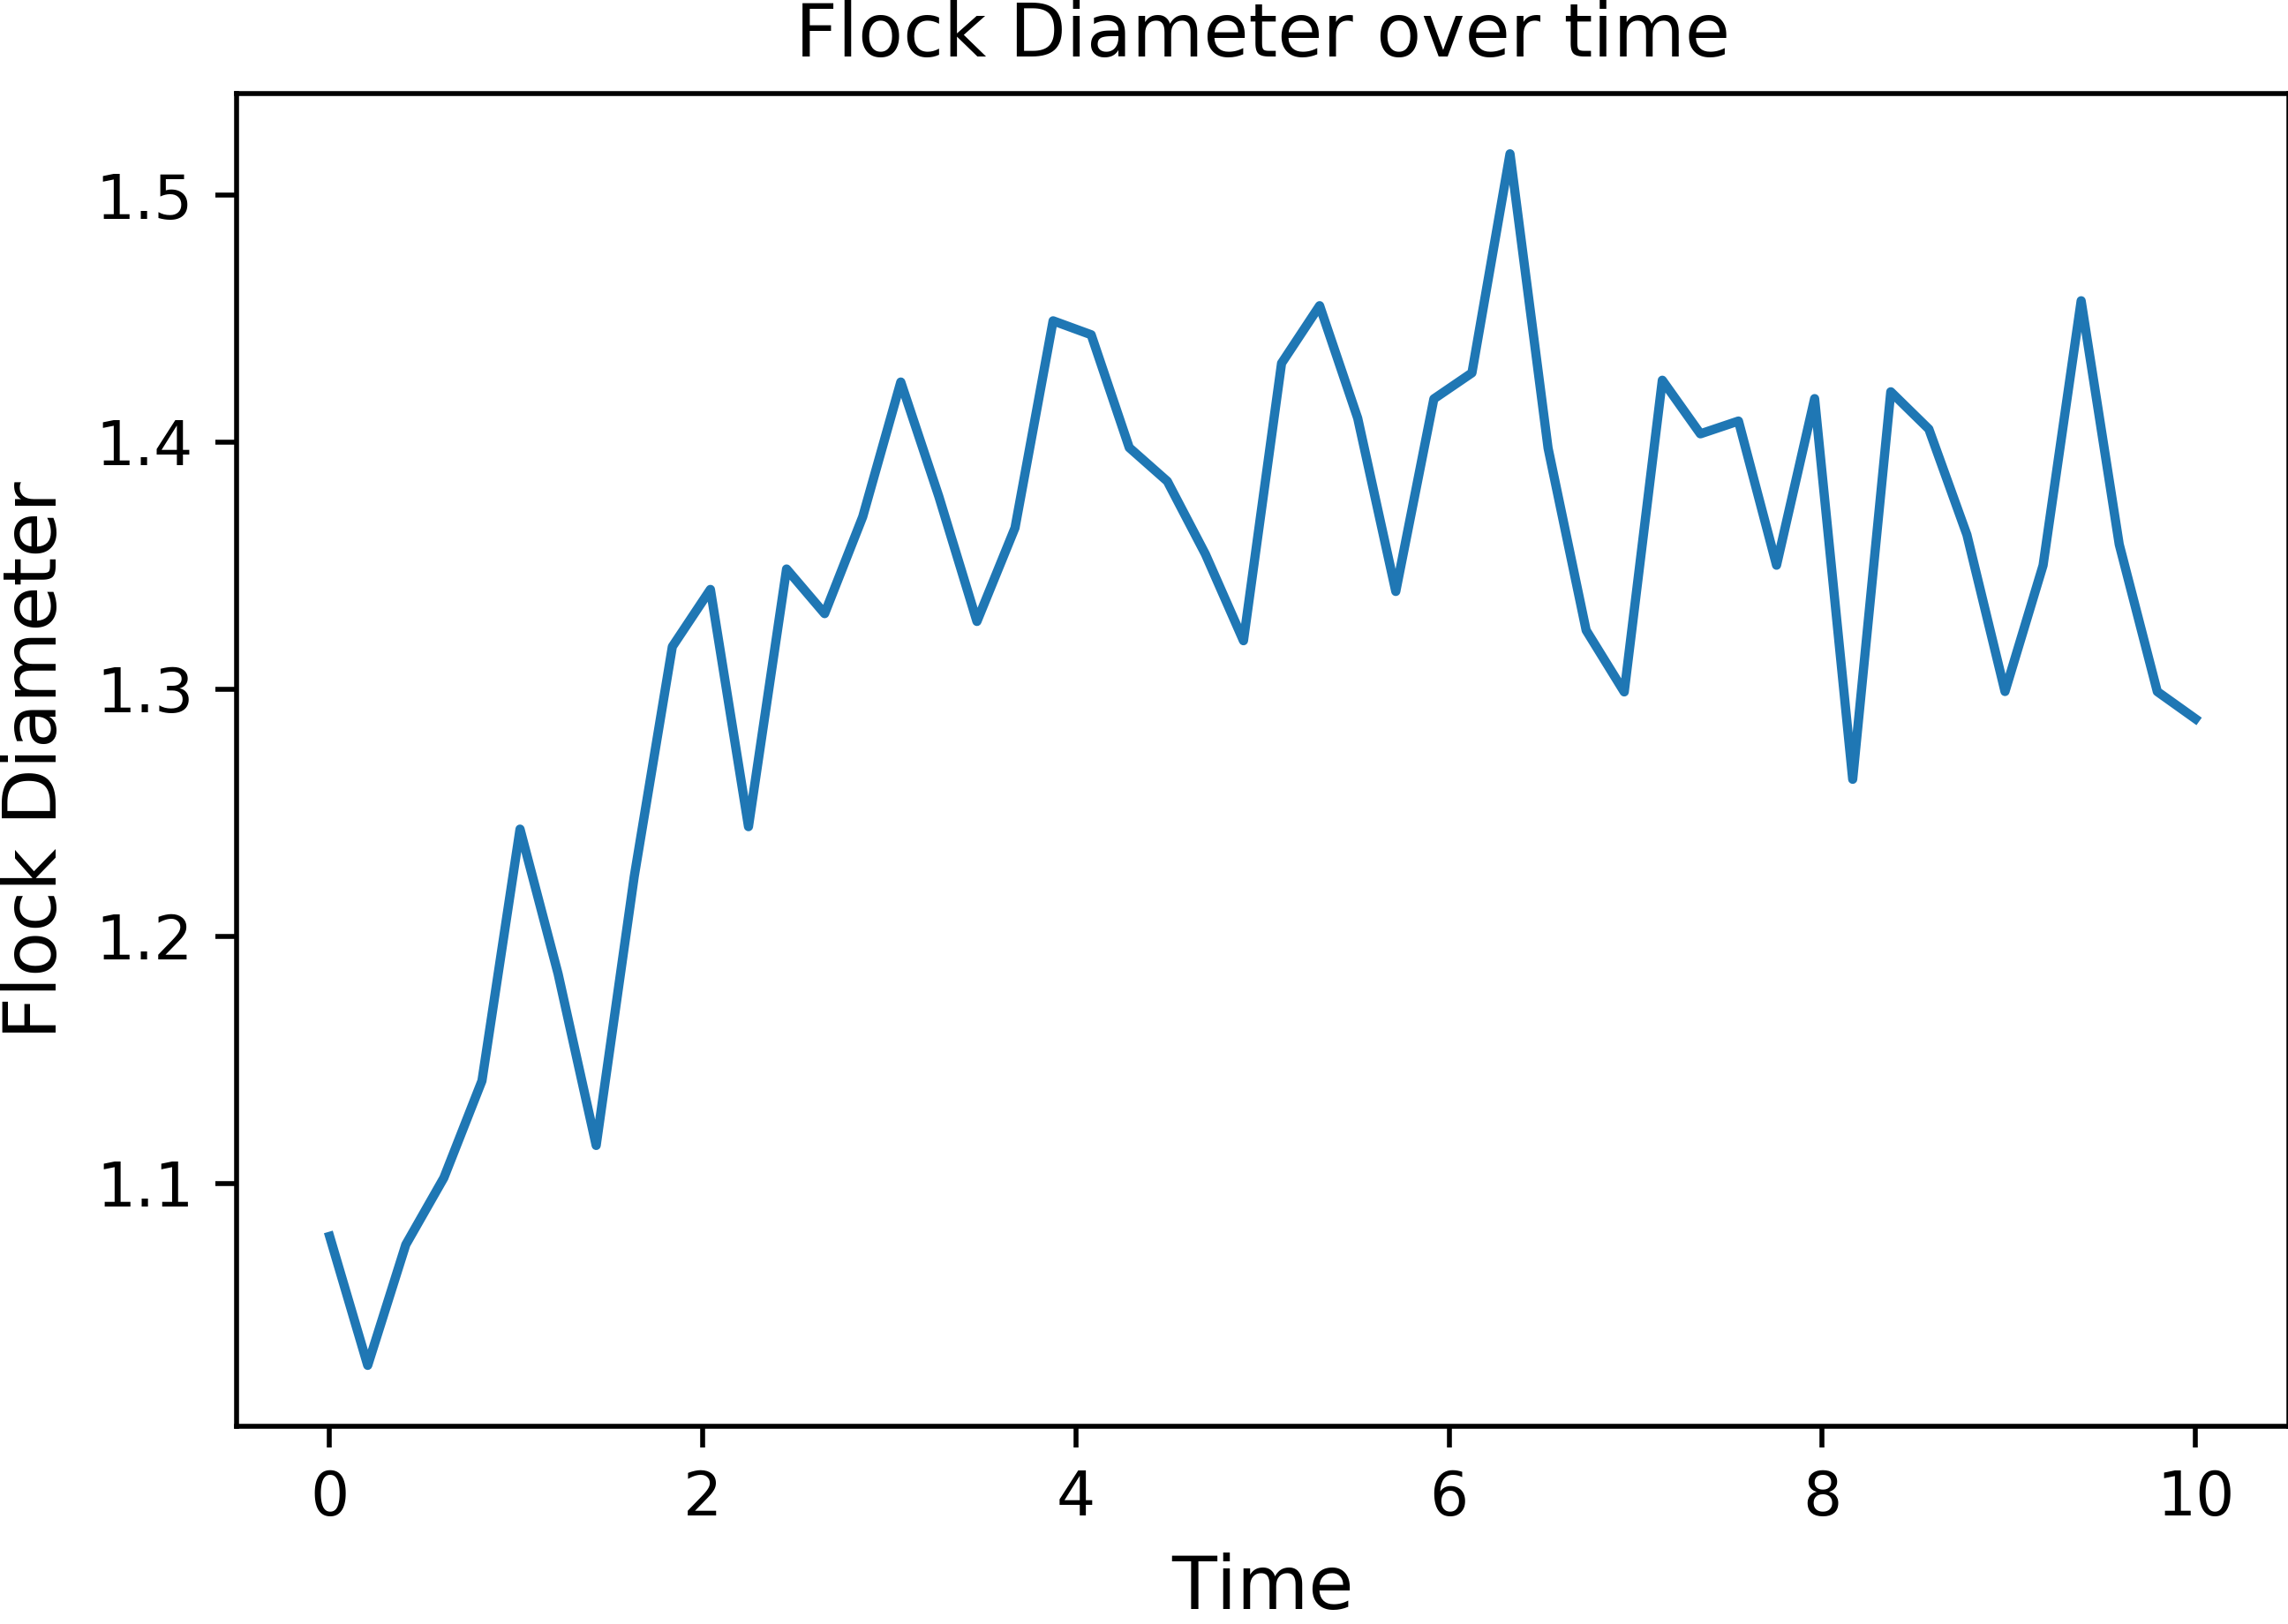
\includegraphics[width=0.85\textwidth]{FlockDiam.png}
        \caption{Flock diameter with $N = 10$}    
    \end{center}
\end{figure}

If we increase the flock size to $N = 30$ and set the food flag to 0, so the food doesn't move, we see
the same behavior in the flock diameter. One can observe this in the visualization \texttt{movie\_2.mp4}.
As time starts the bird are initially in a random position. They then move towards the origin where the food is fixed, and stay there.

\begin{figure}
    \centering
    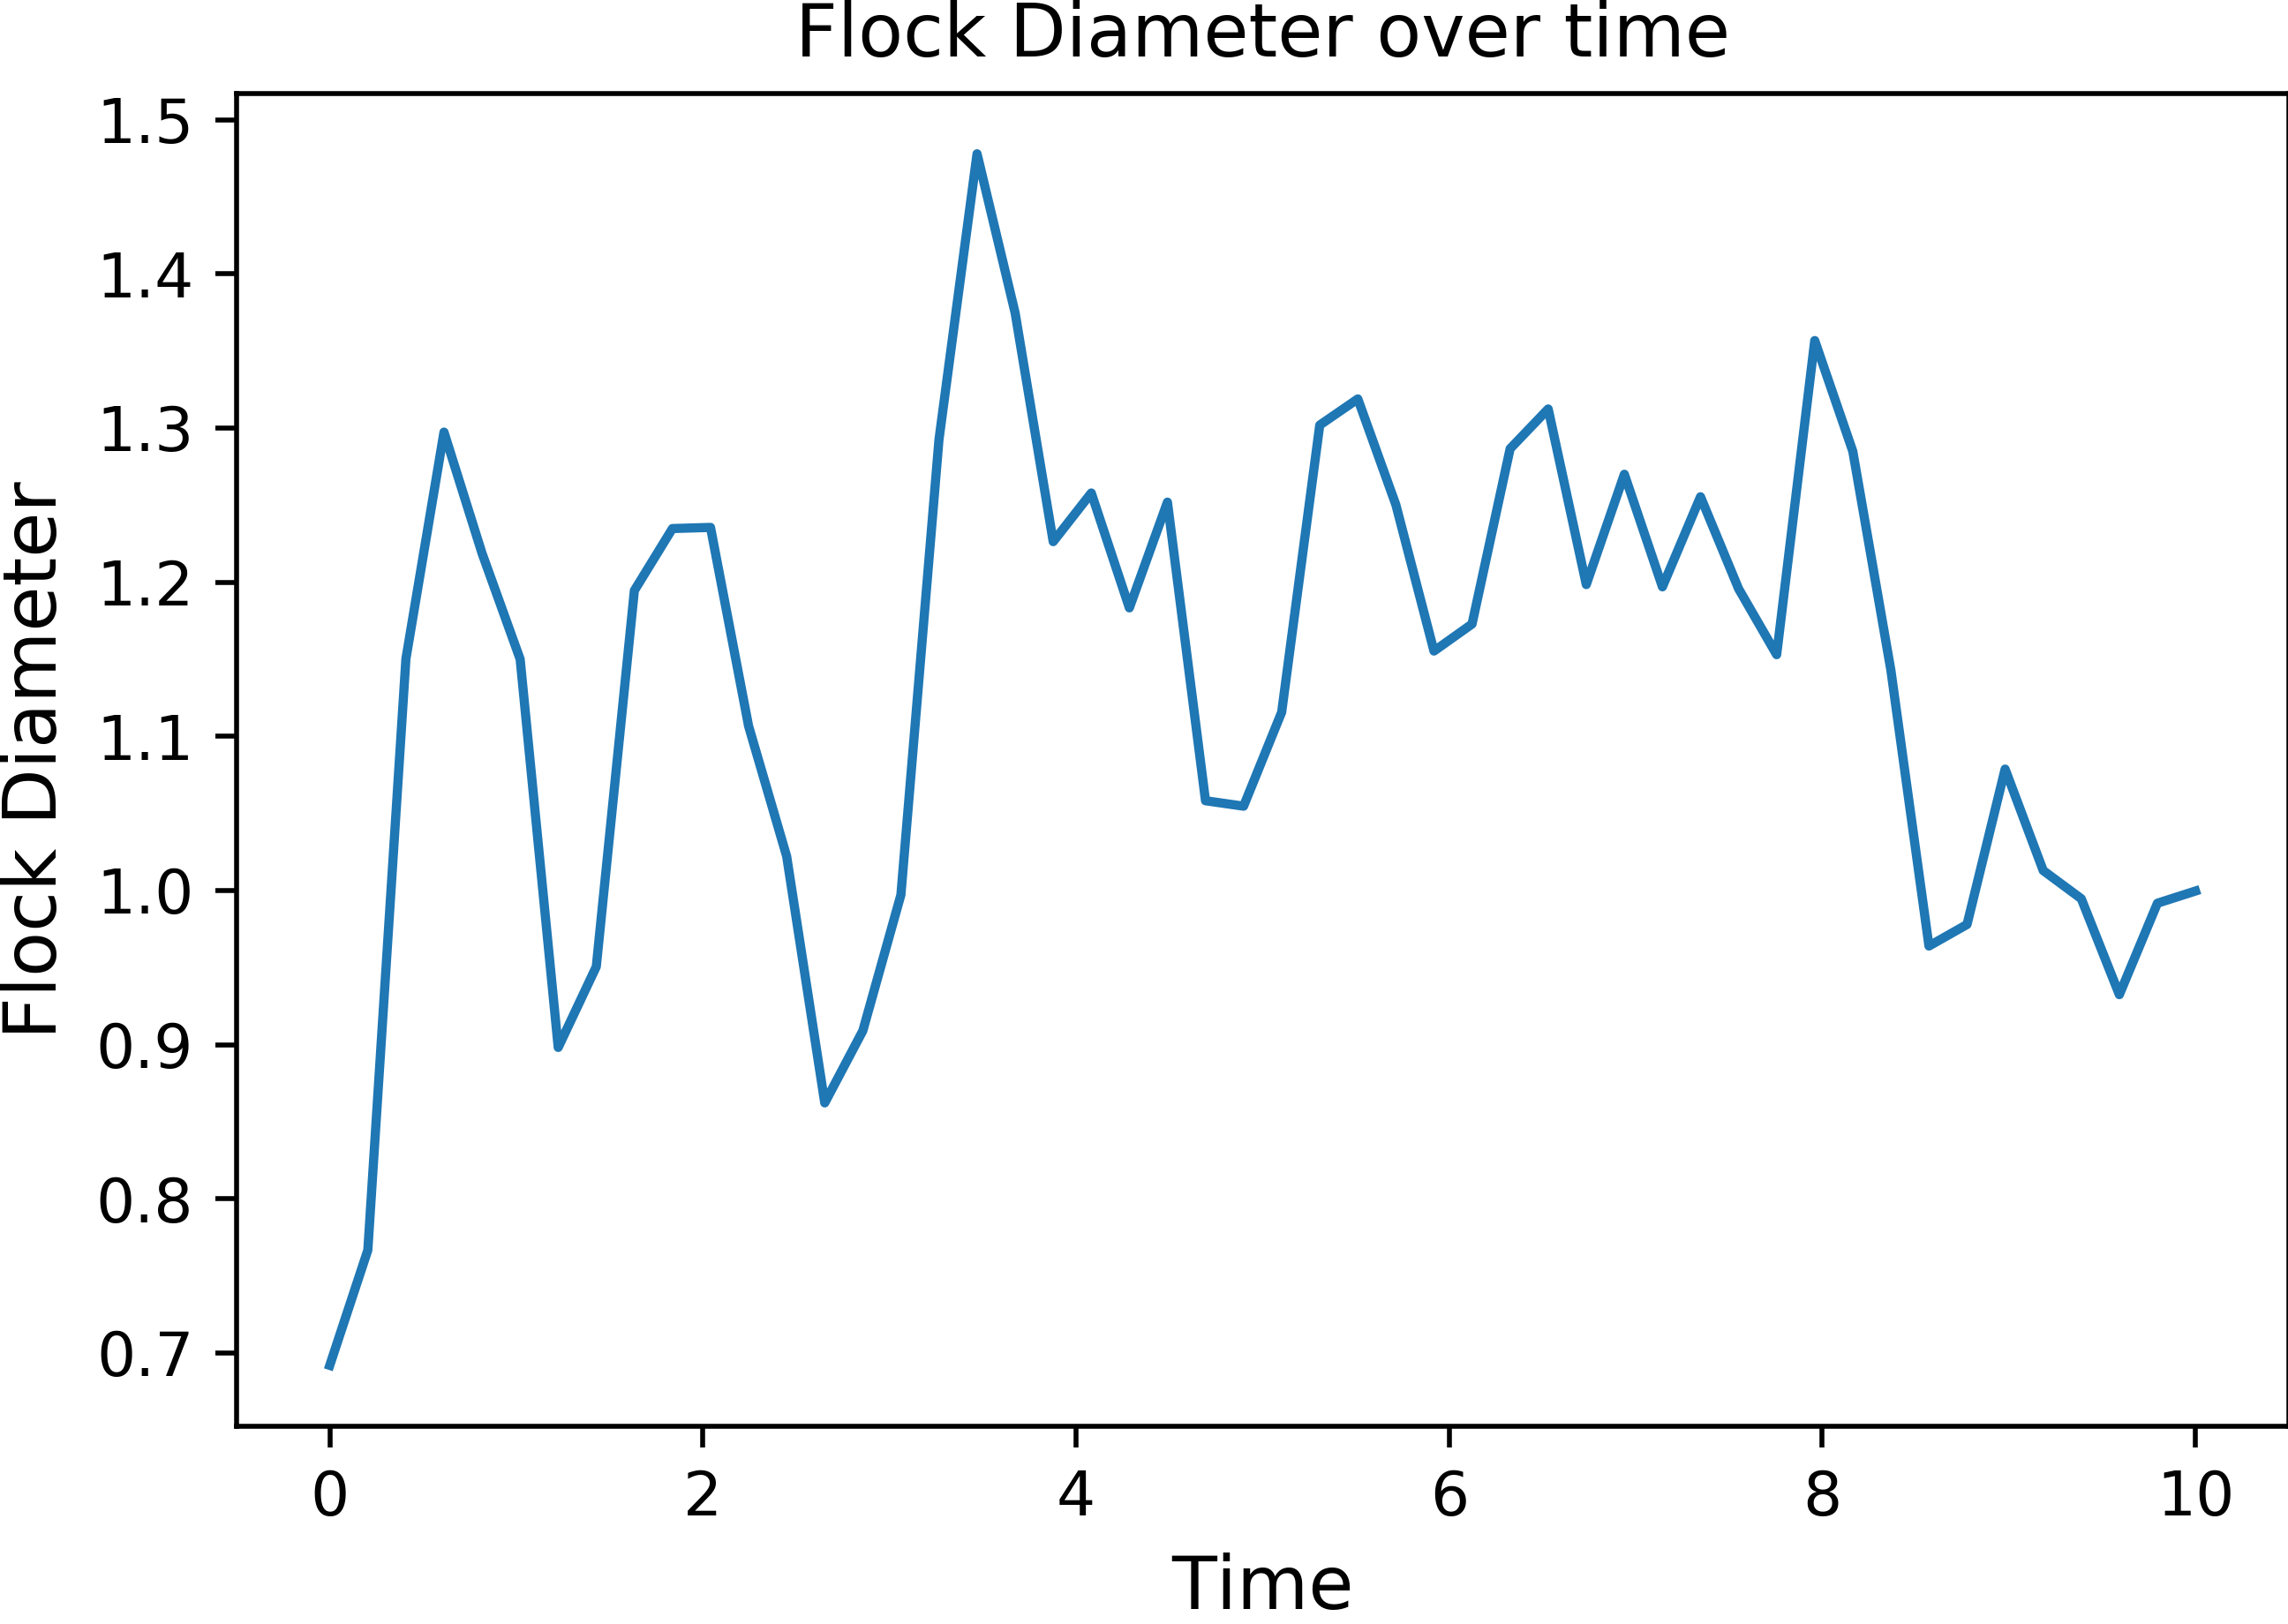
\includegraphics{FlockDiam30.png}
    \caption{Flock diameter with $N = 30$}
\end{figure}
\subsection{Analysis of flock diameter under altered parameters}

Now We'll alter some of the other parameters and see how this affects the size of the flock.
Let's begin by increasing the repelling force from $\rho = 2$ to $\rho = 4$. We'd expect to see an increase in flock diameter, which we certainly do. We also see a much wilder variation in it as well. This is visualized in \texttt{movie\_3.mp4} with flock size $N = 30$ and $C(t) = (0,0)$.

\begin{figure}[h]
    \centering
    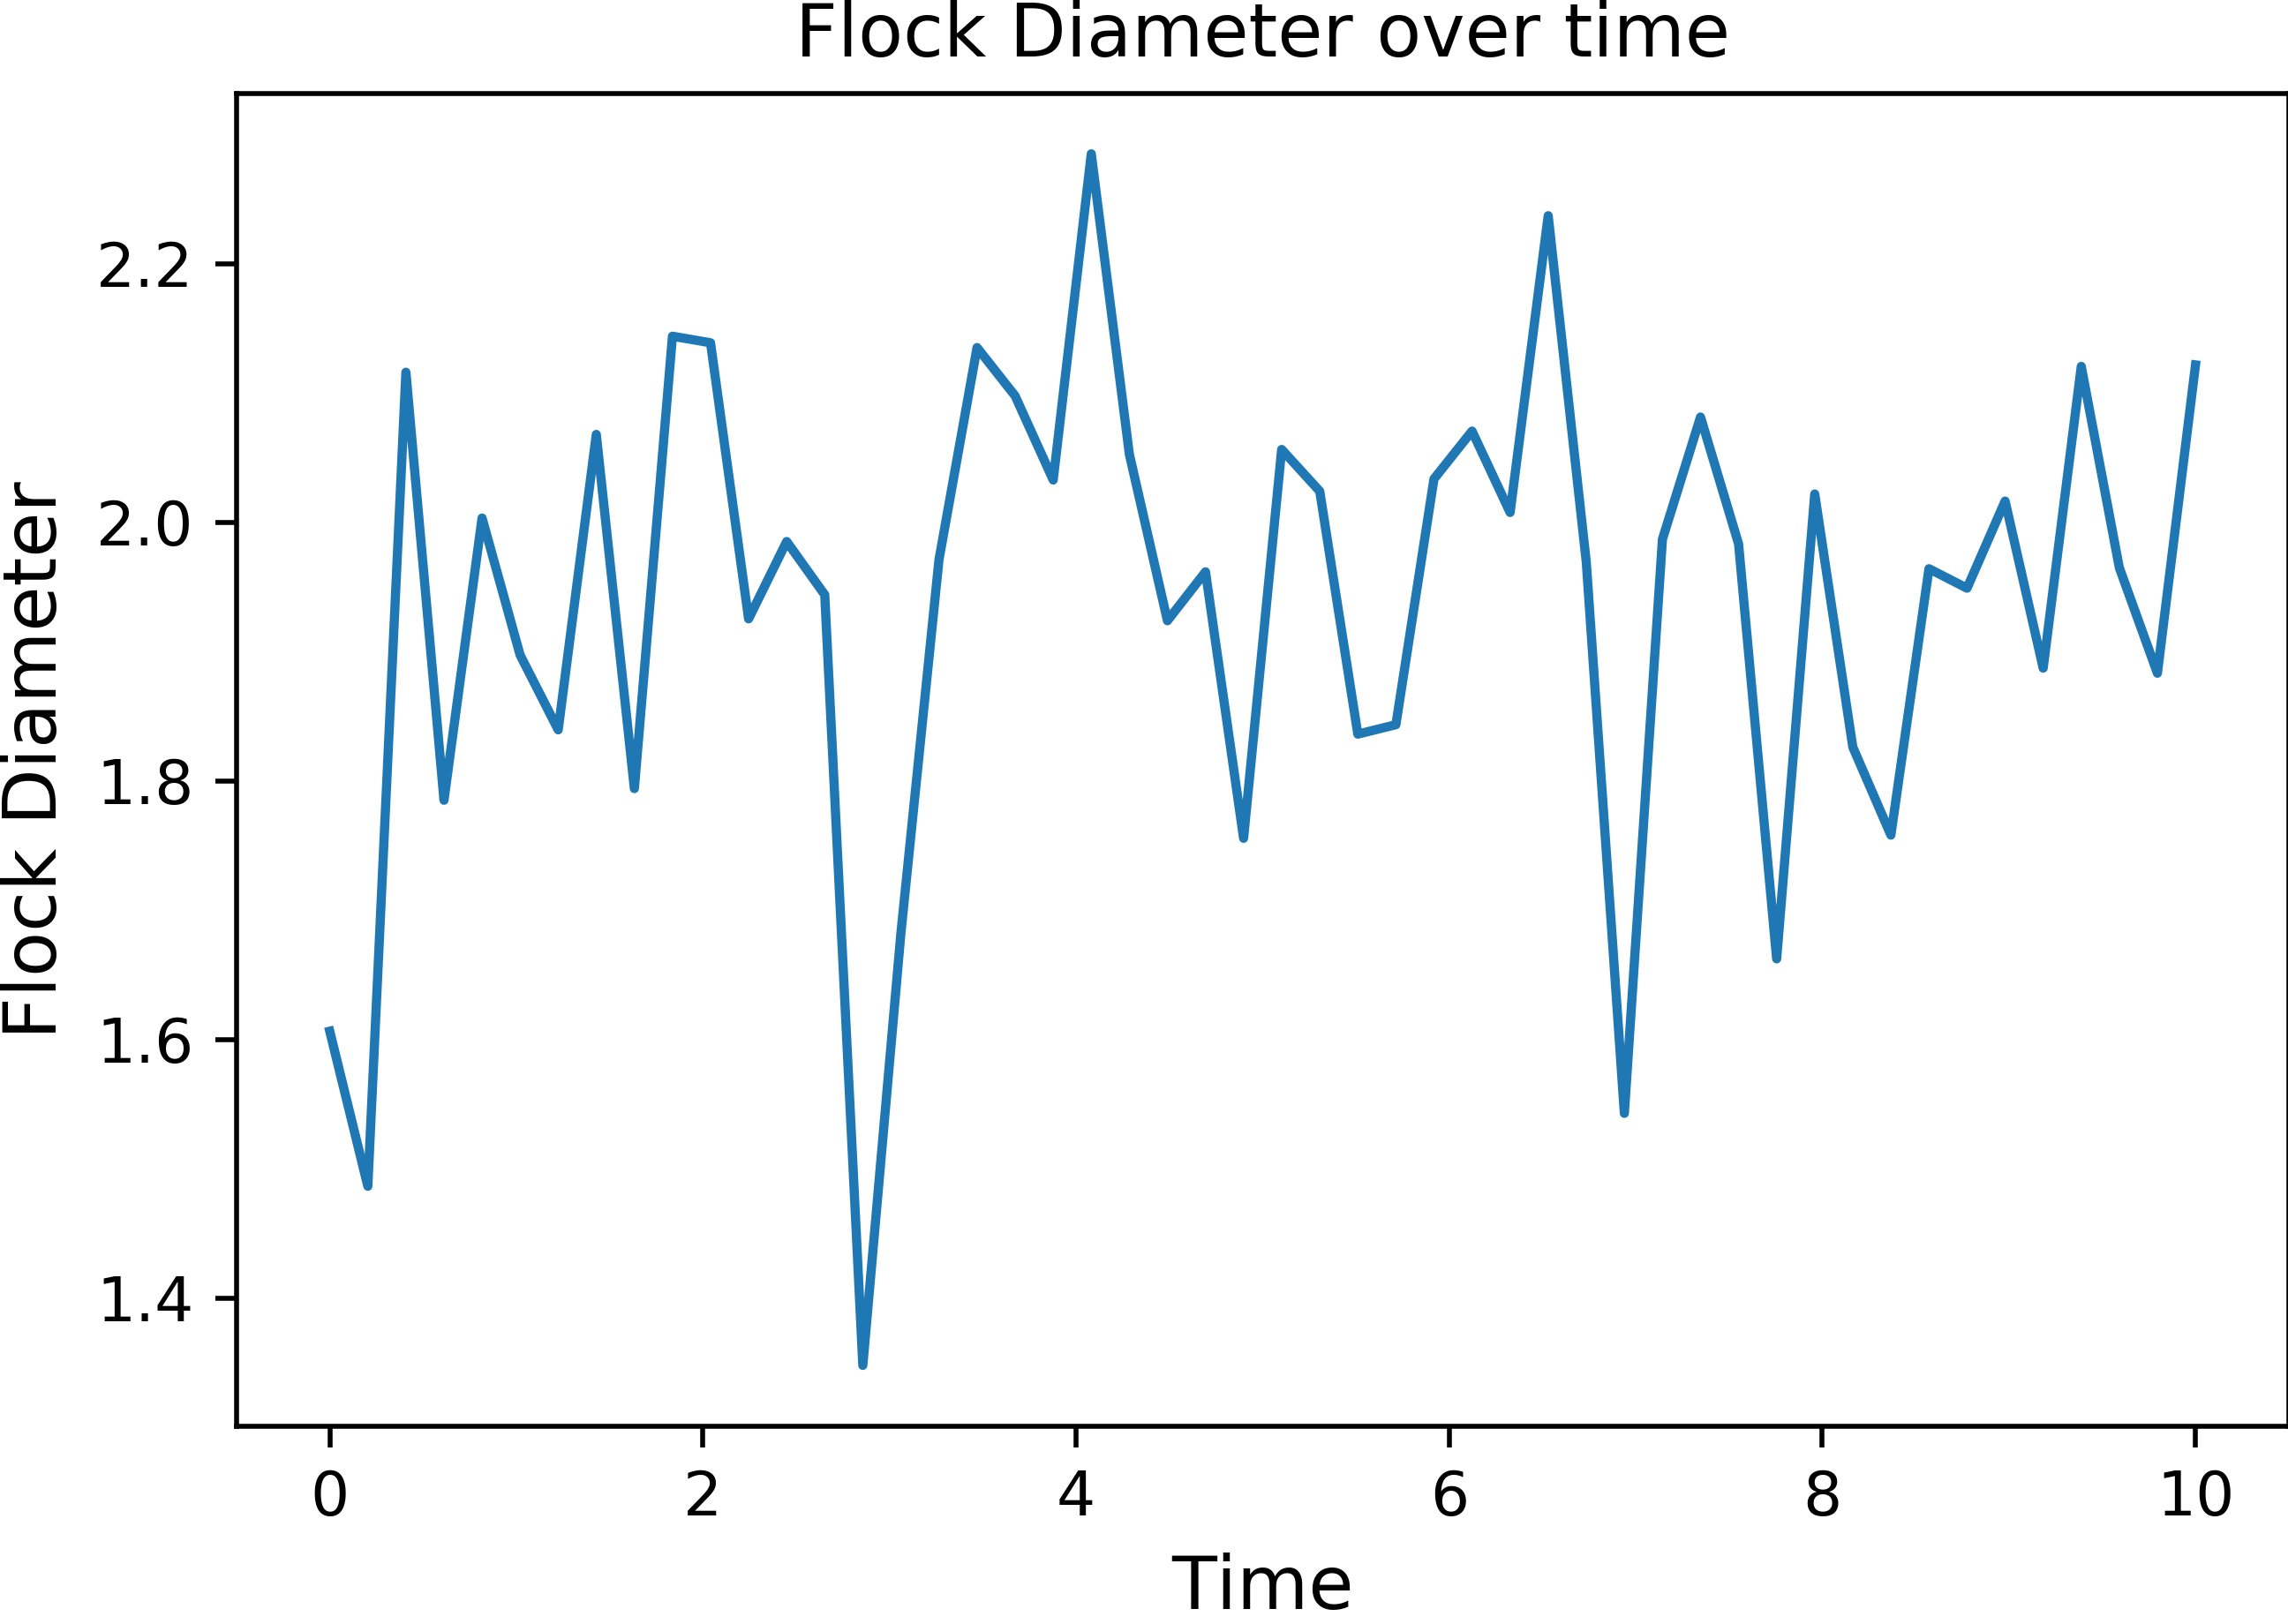
\includegraphics[width = 0.85\textwidth]{FlockDiam30v2.png}
    \caption{Flock diameter with increased repelling force}
\end{figure}

Now let's increase a few other parameters as well. We will keep the value of $\rho = 4$ and we'll increase the flocking force from $\kappa = 4$ to $\kappa = 5$ and increase the speed at which the food moves from $\alpha = 0.4$ to $\alpha = 1.4$. We'll also make the lead bird more charismatic and change the value from $\gamma_2 = 8$ to $\gamma_2 = 10$. This scenario is visualized in \texttt{movie\_4.mp4}.

If we increase the flock size in this scenario from $N = 30$ to $N = 100$, the problem becomes unstable. To solve this system with a larger flock size, we increase the number of time steps from 50 to 100. This is visualized in \texttt{movie\_5.mp4}.

\section{Conclusion}
Through experimentation, it was discovered that certain parameters, if too great, would cause the flock to disperse. The flocks size also plays a roll in how many time steps we need to find an accurate solution. It was also noted that some birds would find a "sweet-spot" where it seems like various force would balance, and their relative locations would remain consistent.
\end{document}
